\chapter{Development}~\label{cha:development}
Development of the application was divided into two main parts: the frontend and the backend, with the backend further broken up into its constituent services. The entire project was maintained in a single mono-repository, with each backend service and the frontend housed in separate directories. While this is not necessarily the optimal structure for a larger project, this approach reduces overhead for a project of a smaller scope, making it the most practical solution.

\section{Frontend}~\label{sec:frontend-development}
\subsection{Implementation}
The actual implementation of the frontend used Vite as a development server and build tool for the React frontend. Vite gave a starting TypeScript template, which was modified to create the application.

Once the build system was in place, the design was broken into components that could be built independently. The HeroUI component library used in this project provided basic components common to most web applications, such as buttons, modals, and input fields. From these, more complex components could be built. One of the benefits of using this component library was its integration with Tailwind CSS, which allowed for stylings to be applied through class names rather than bespoke stylesheets, significantly reducing the time needed to style the application and ensuring a consistent look across the application.

After completing the frontend components, the next step was integrating the frontend with the backend services. Some functionalities of the application required user authentication through Spotify to access Spotify API features. This had to be implemented on the frontend using Spotify’s OAuth2 flow~\cite{SpotifyOAuth}, which redirects the user to Spotify for login and then returns them to the application with an access token in the URL. Once redirected the application reads the access token and saves it to local storage to be used in subsequent requests to Spotify.

Once the authentication was implemented, all endpoint calls to the backend were implemented as functions that could be imported and run by any component. The requests were made using the Axios library, which, though not a native JavaScript library, is widely used and well-documented, making it easy to implement.

\subsubsection{Landing Page}
An oversight in the original design was the lack of a landing page presented to users before logging in. The page follows the application's stylings and contains graphics and text related to the application. Once the user logs in, they are redirected to the application's main screens. A landing page also briefly overviews the application and its features and adds visually appealing graphics, which might improve the user's initial impression of the application.

\begin{figure} [H]
    \centering
    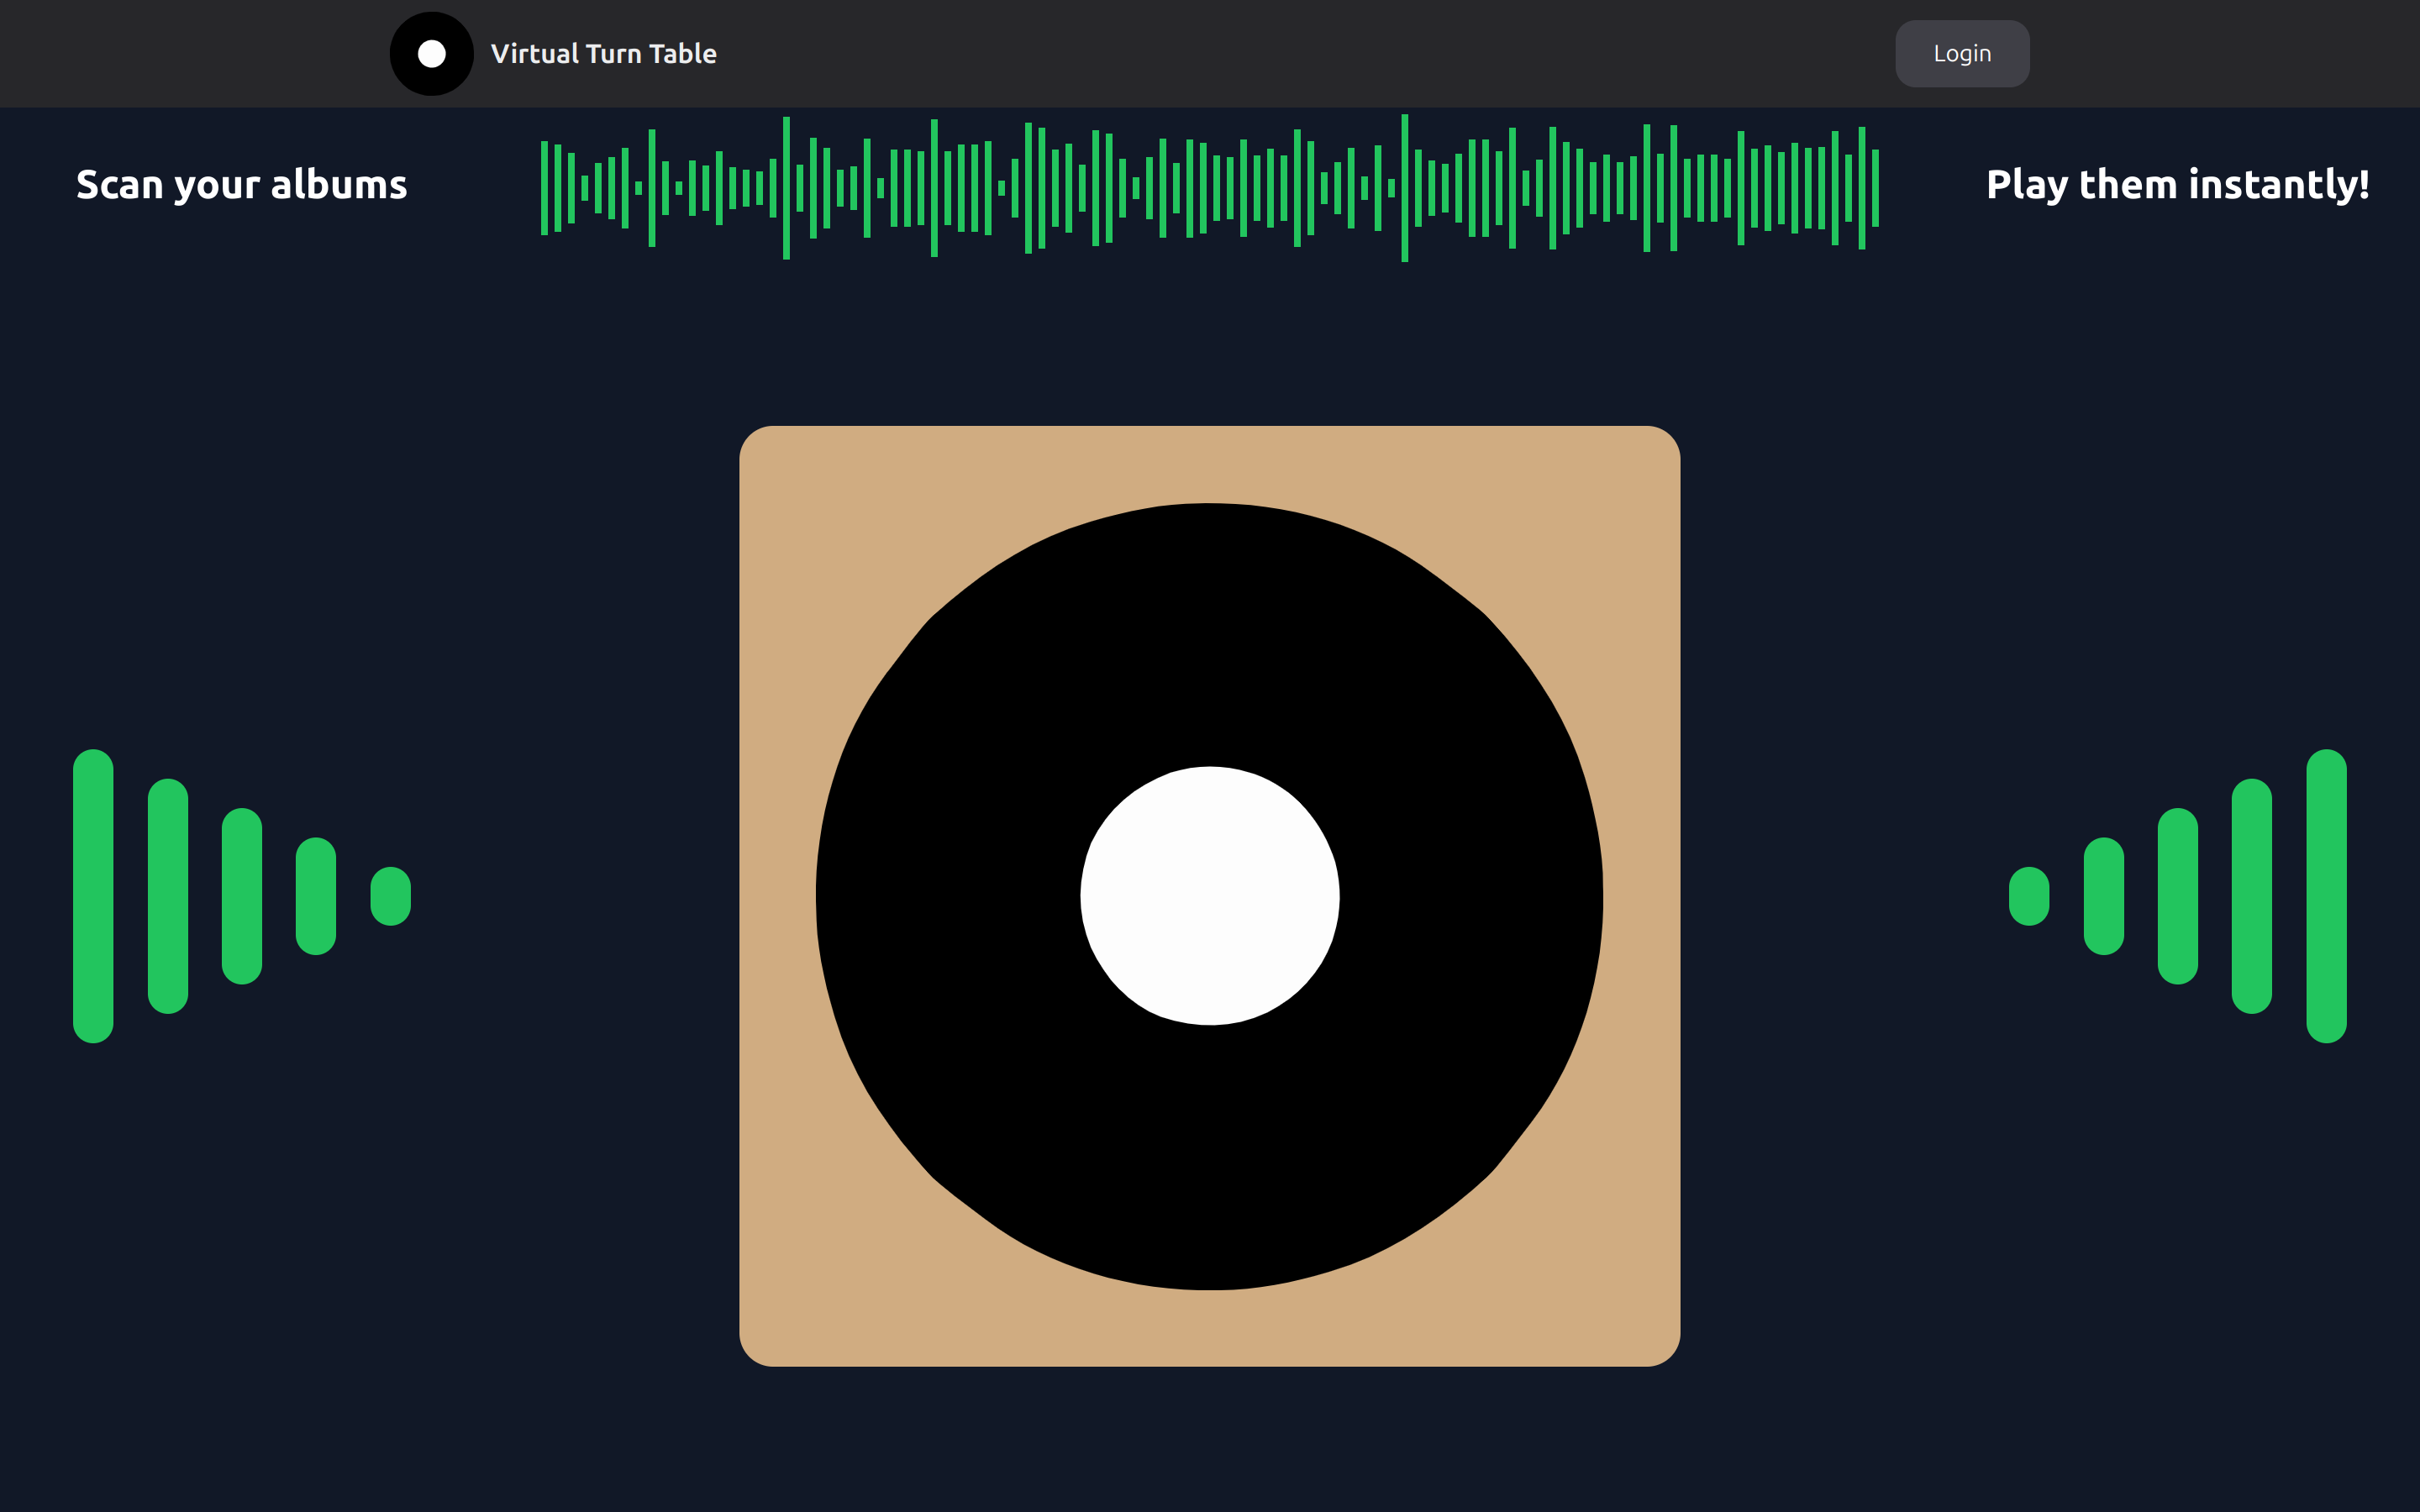
\includegraphics[width=0.8\textwidth]{figures/landing_page.png}
    \caption{The landing page of the application}
    \label{fig:landing_page}
\end{figure}

\subsubsection{Navigation Bar}
The navigation bar is a component included on all screens, which allows the user to navigate between the different screens of the application. It has a static logo, screen selection tabs, and user details. The user details also serve as a dropdown trigger which displays a menu, as seen in Figure~\ref{fig:user_options_menu}, with account options such as setting their collection to public, sharing their collection with a specific user, deleting their account, and logging out.

\begin{figure} [H]
    \centering
    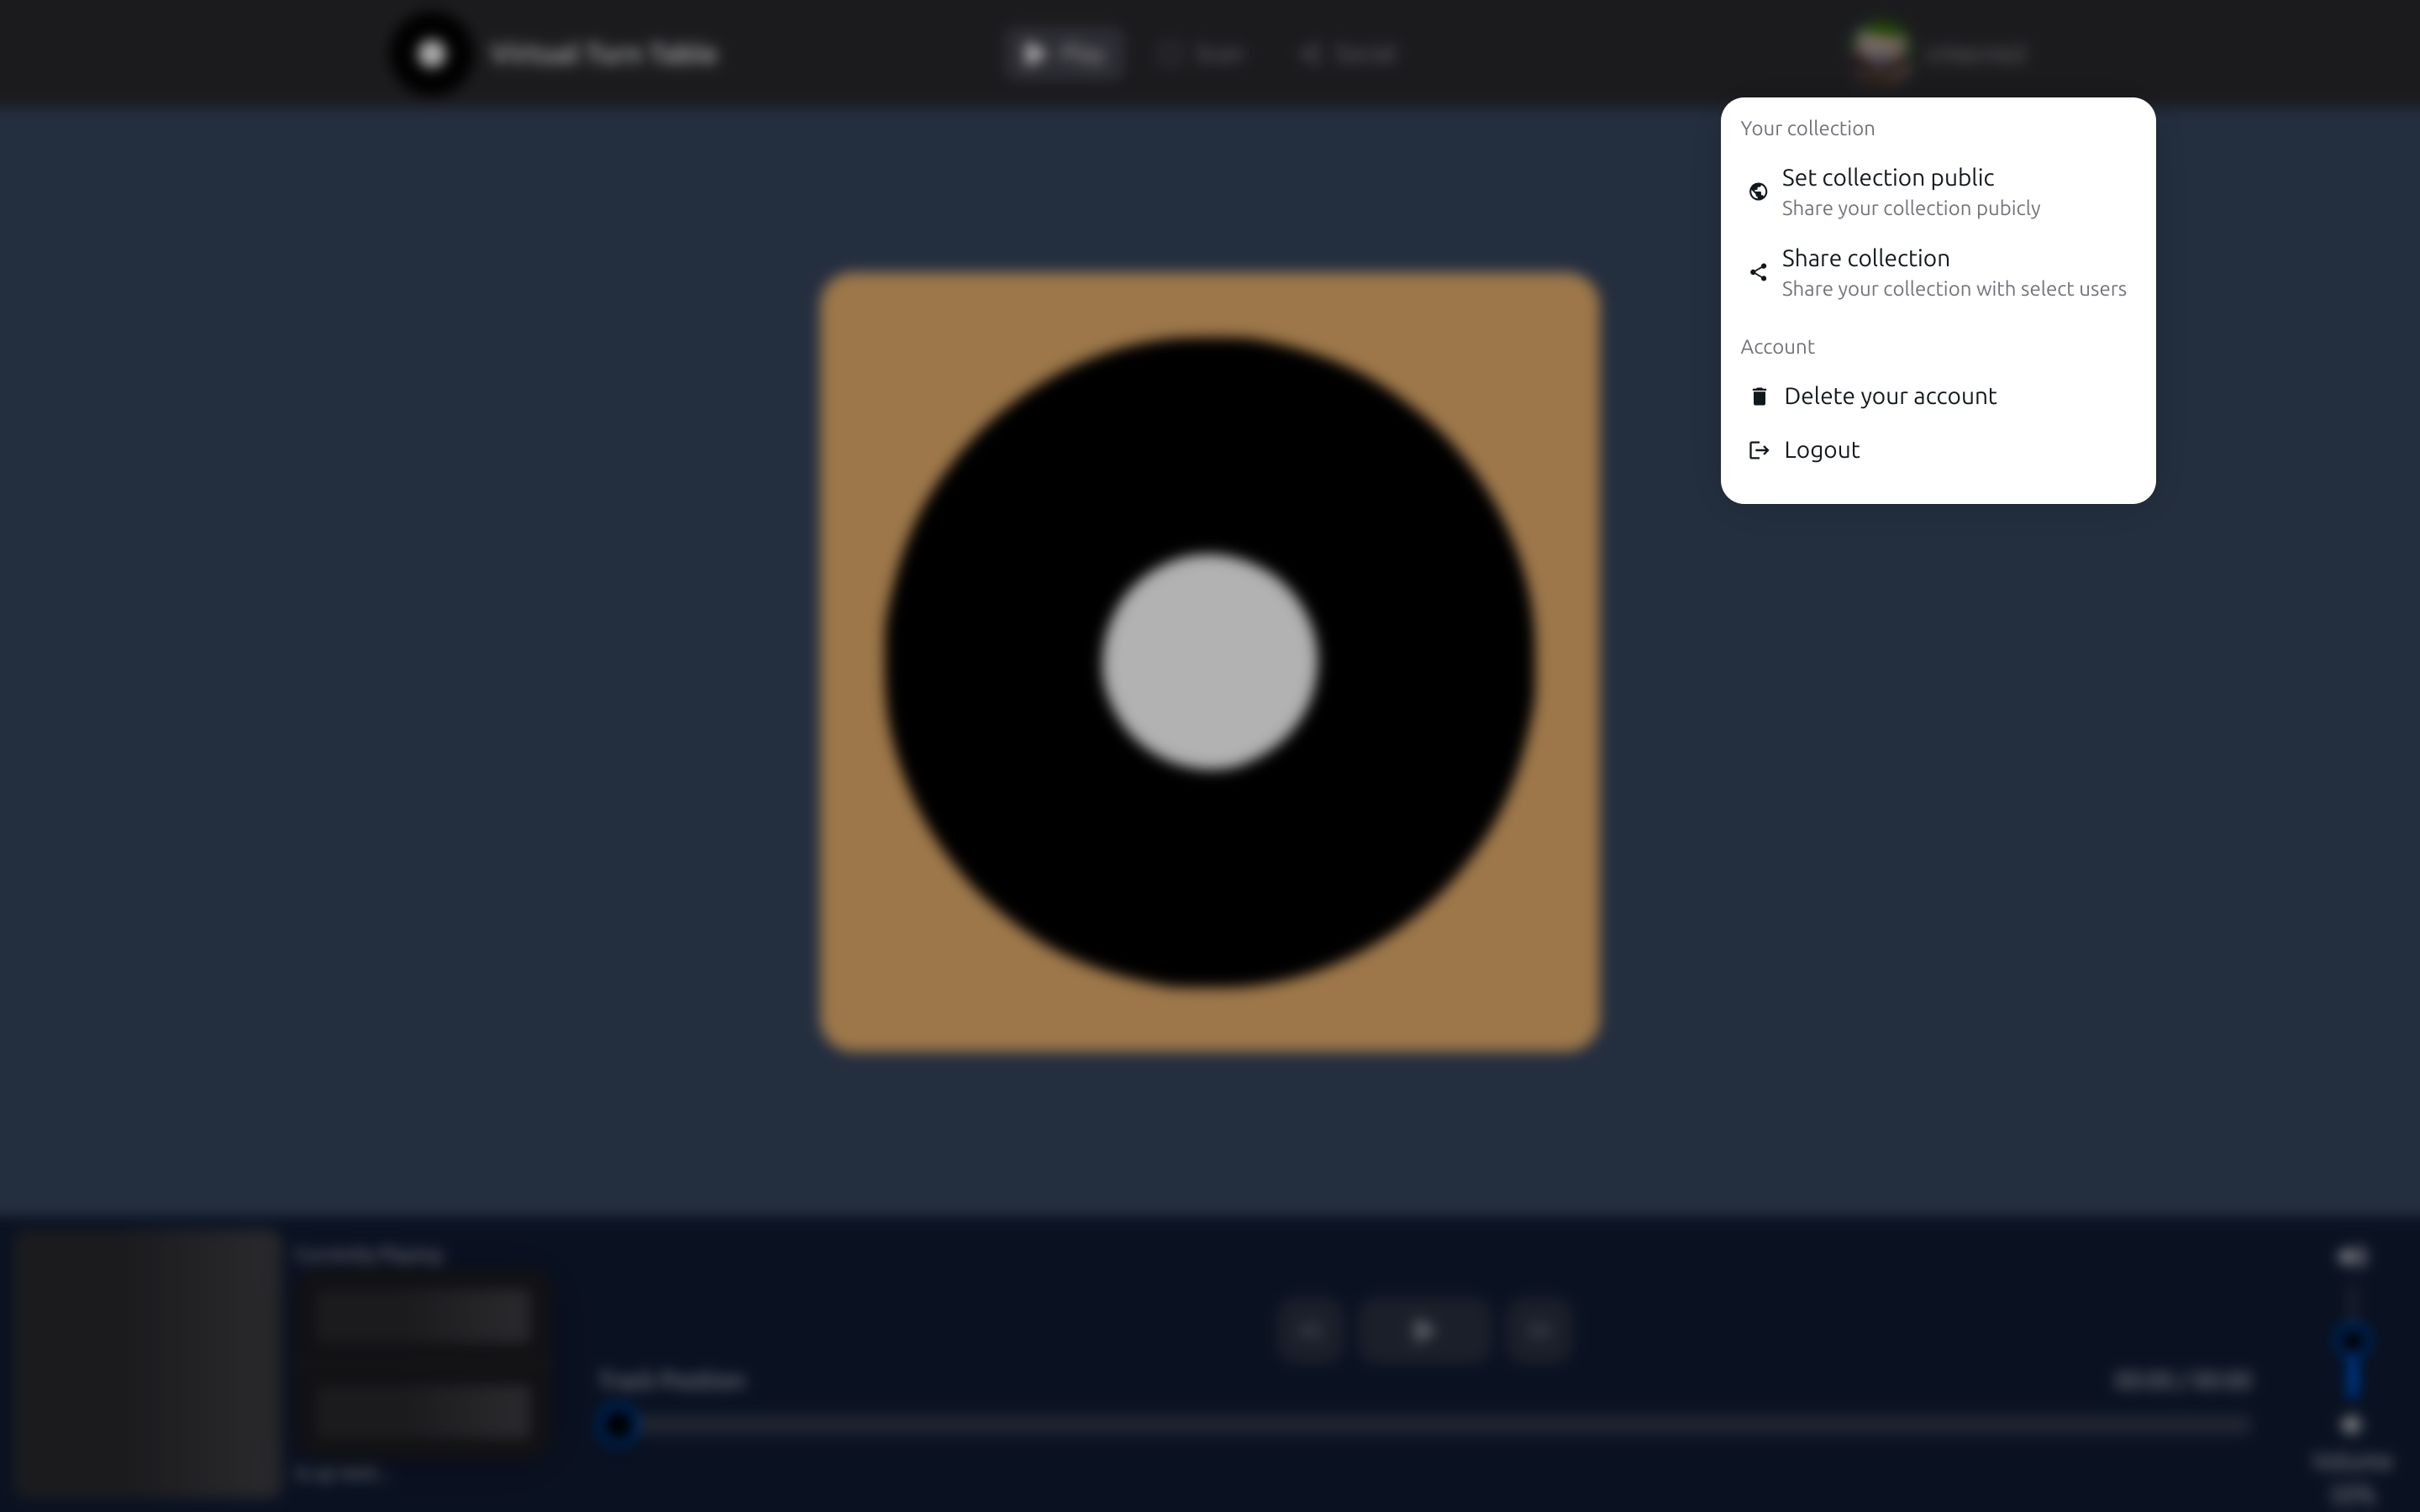
\includegraphics[width=0.8\textwidth]{figures/menu_open_screen.png}
    \caption{The user options menu opened from the navigation bar}
    \label{fig:user_options_menu}
\end{figure}

\subsubsection{Play Screen}
The play screen largely follows the initial design, consisting of three main sections: the track list, the controls, and a spinning vinyl animation. Music playback is handled by the Spotify Web Playback SDK, a client-side JavaScript library that enables real-time control of Spotify playback within the browser. Actions such as changing tracks, skipping forward or backwards, and pausing are executed by invoking the corresponding methods provided by the SDK.

\paragraph{Track List}
The track list displays all tracks from the currently active album set on the scan screen. It serves as a selection menu of tracks, allowing users to choose a specific song for playback, similar to a music streaming service. The component is styled to fill up all vertical space between the navigation bar and scrolls vertically if the number of tracks exceeds the available space.

\paragraph{Controls}
The playback controls consist of buttons and sliders that users can interact with to affect audio playback. Clicking a button or adjusting a slider calls the relevant SDK methods, allowing users to play, pause, skip, or adjust volume. Album art and track information are displayed so the currently playing track can be easily identified. These automatically update as the active song changes.
One feature from the original design was removed: the ability to scrub through the whole album rather than only the currently playing track. This was considered too complex to implement and added little to the user experience, so it was excluded from the final implementation.

\paragraph{Spinning Vinyl}
Several animations were added to the application to emulate the feel of a physical record player. This includes the spinning vinyl animation here, which acts like a vinyl on a traditional turntable, starting and stopping as the music is played and paused. The effect is achieved by editing the CSS rotation of the graphic at set intervals, which, as it is done frequently enough, makes it look like a smooth rotation.

Alongside the spinning, a second animation was added to simulate the act of removing the vinyl from its sleeve when changing albums. When an album changes, the vinyl disc appears to be pulled out of its sleeve before the music begins playing. The effect was achieved similarly to the spinning with CSS animations moving an image of the vinyl sleeve off the screen to reveal the vinyl graphic underneath.

\begin{figure} [H]
    \centering
    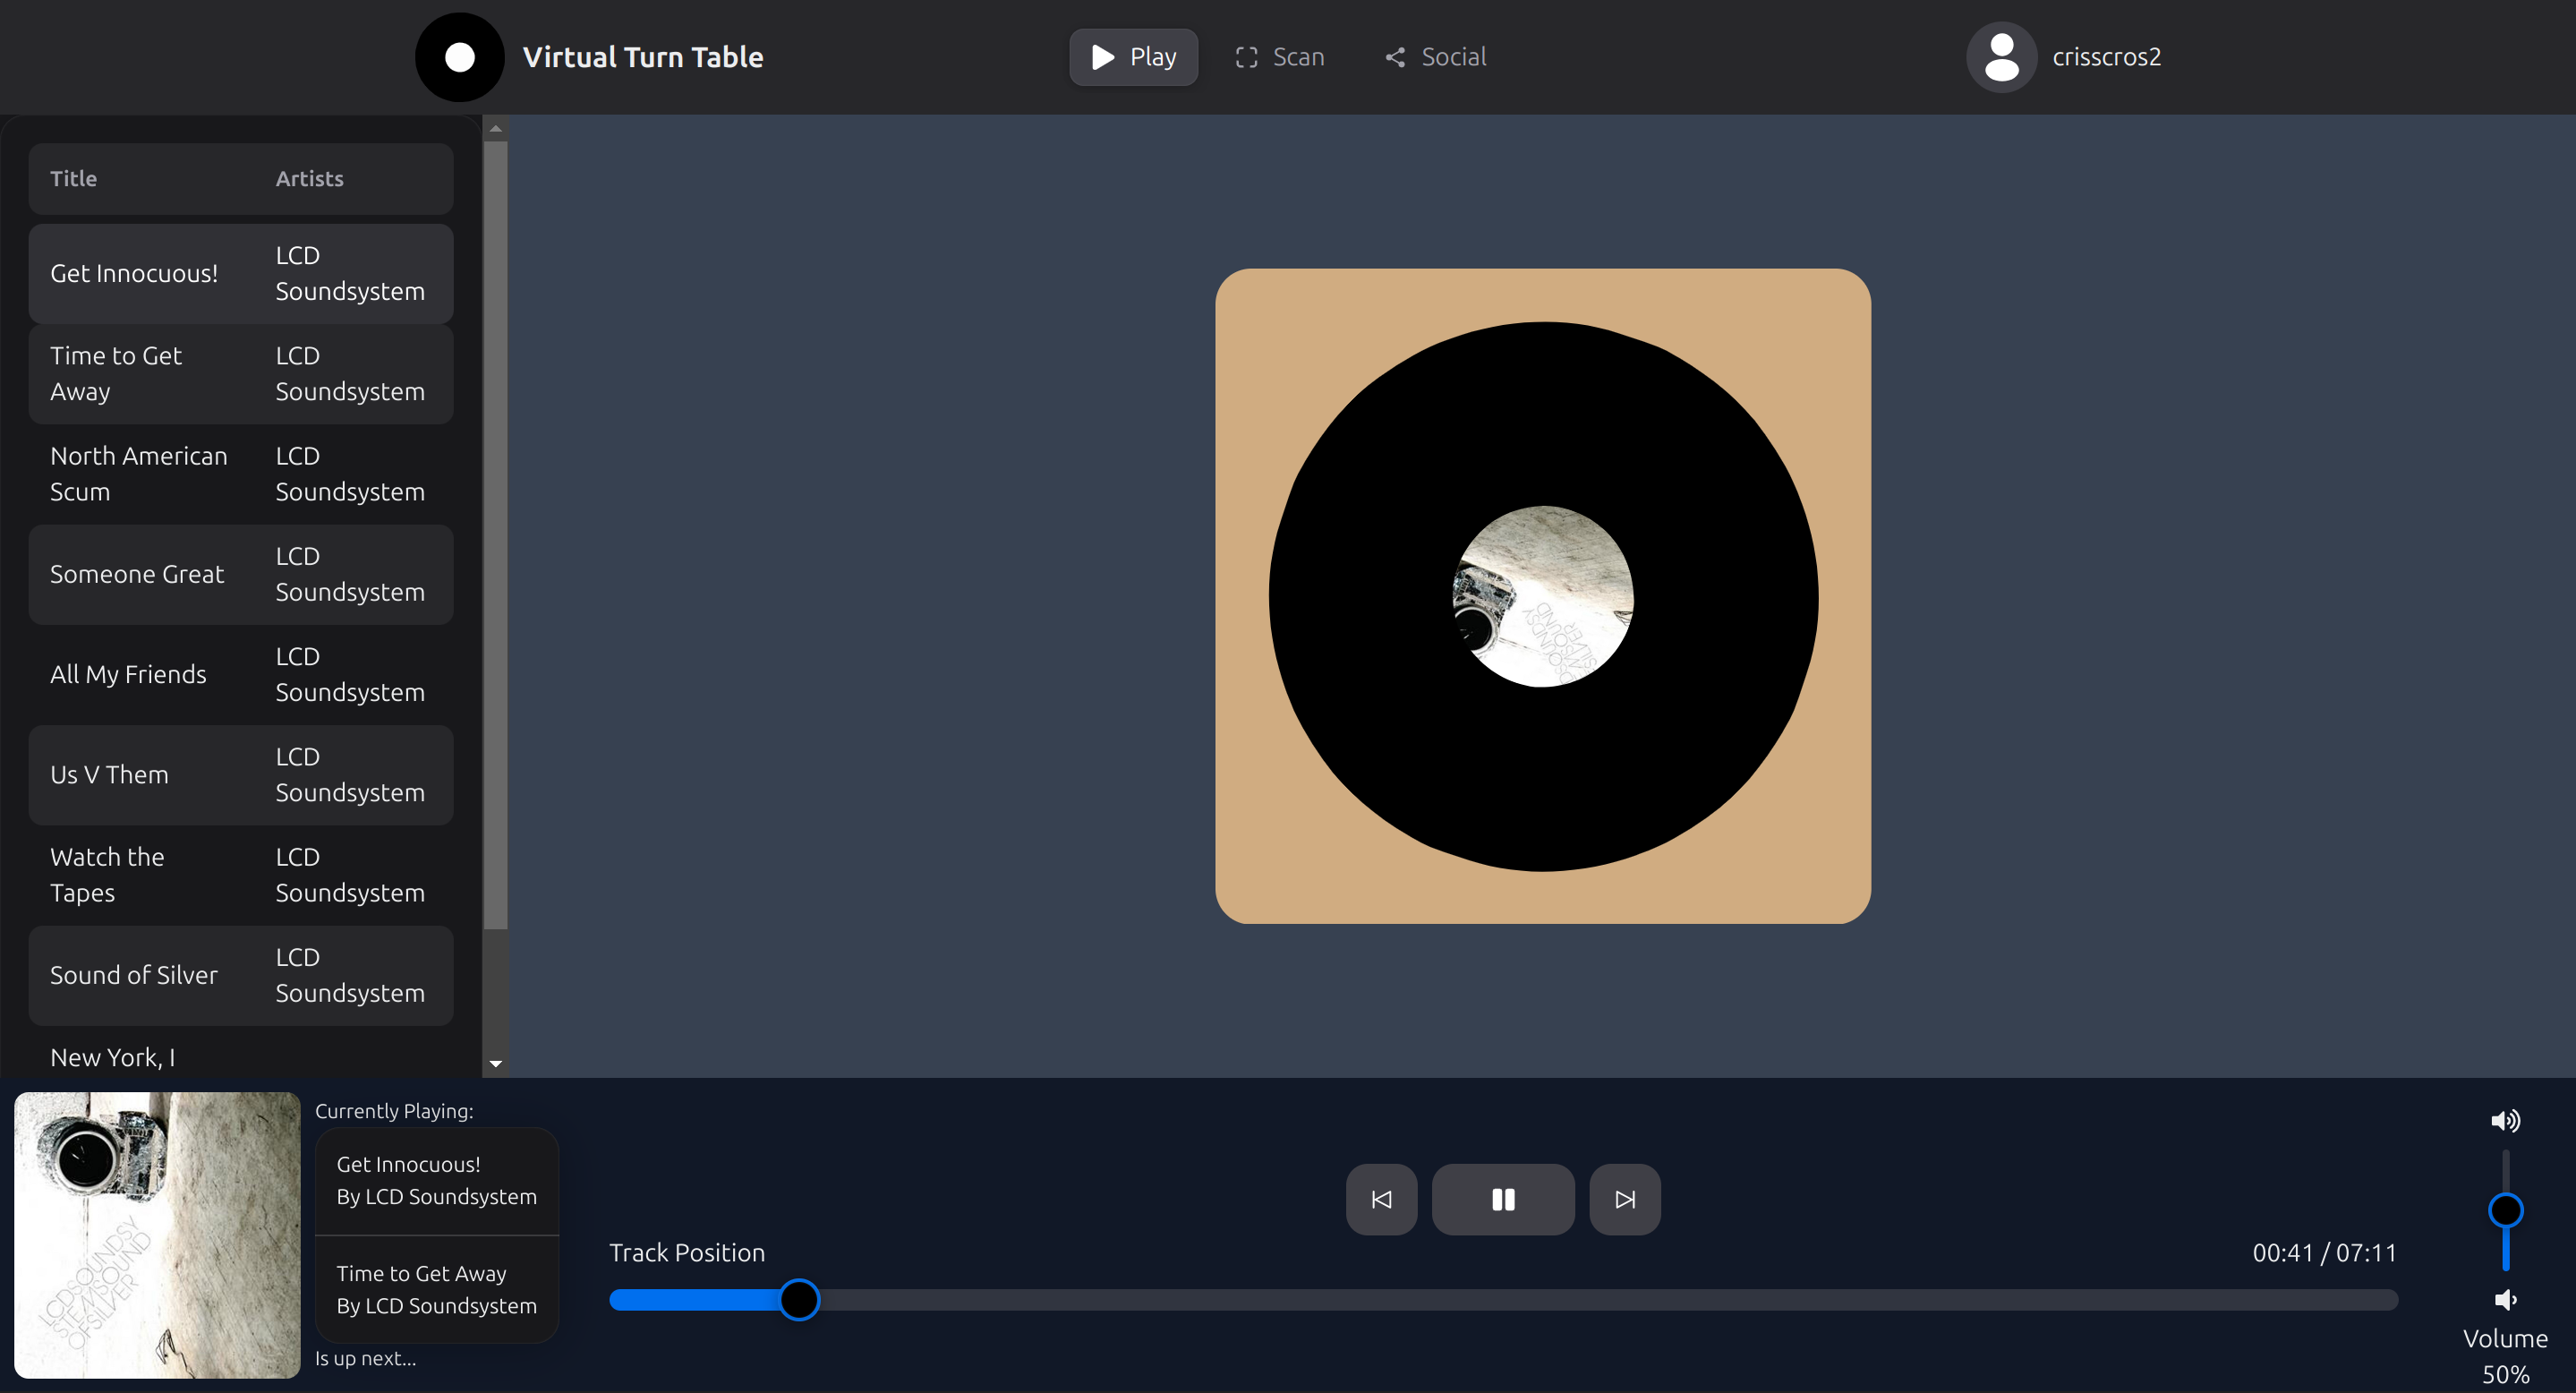
\includegraphics[width=0.8\textwidth]{figures/play_screen.png}
    \caption{The play screen of the application}
    \label{fig:play_screen}
\end{figure}

\subsubsection{Scan Screen}
The scan screen, though following the initial design as closely as possible, had to be changed during development as some issues with the original design became apparent. Similarly to the play screen, it was also split into three main parts: the album confirmation sidebar, the scan section, and the album collection.

\paragraph{Album Confirmation Sidebar}
The album confirmation sidebar allowed the user to confirm that the identified album was correct. However, the fact that this only showed a single album presented an issue that was not addressed in the original design: how to handle incorrect album identifications. The solution was a second stage of the confirmation, using a separate scattershot approach to present alternative matches, as shown in Figure~\ref{fig:album_confirmation_sidebar_incorrect}. In addition, the sidebar also acts as a method to display to the user the application is processing through a loading animation where the identified album will appear. Once the user confirms the album selection, the sidebar slides back to the side of the screen, and the album is set as the active album on the play screen.

\begin{figure}[H]
    \centering
    \begin{subfigure}[t]{0.3\textwidth}
        \centering
        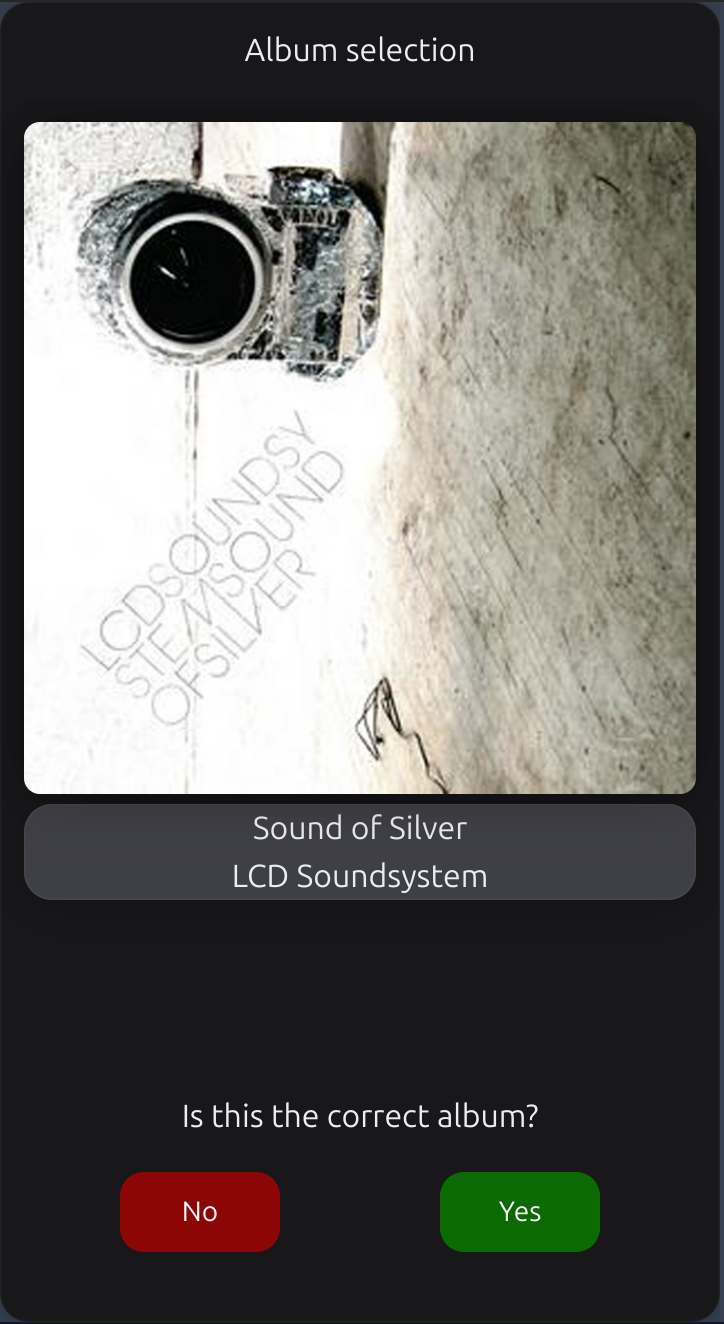
\includegraphics[width=0.8\textwidth]{figures/corrent_album_confirm.png}
        \caption{The album confirmation sidebar with the correct album guessed}
        \label{fig:album_confirmation_sidebar}
    \end{subfigure}
    \begin{subfigure}[t]{0.3\textwidth}
        \centering
        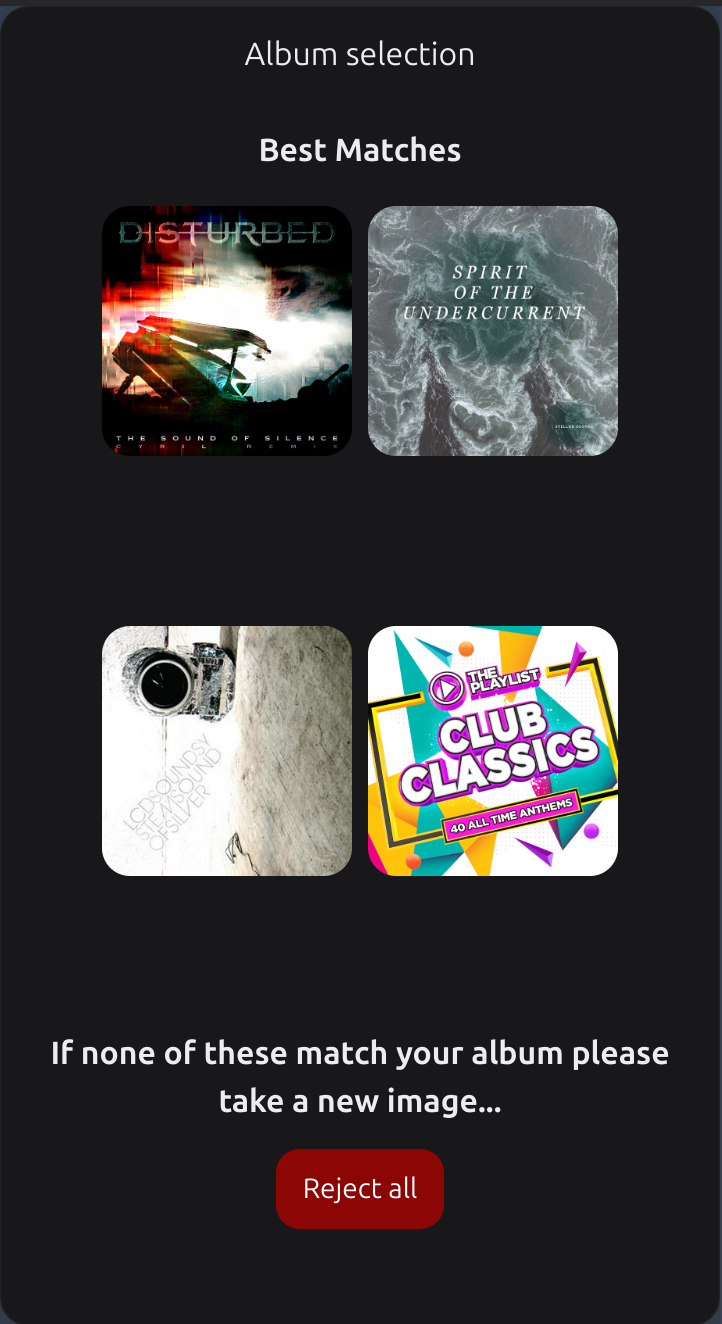
\includegraphics[width=0.8\textwidth]{figures/top_results_confirm.png}
        \caption{The album confirmation sidebar with the incorrect album guessed}
        \label{fig:album_confirmation_sidebar_incorrect}
    \end{subfigure}
\end{figure}

\paragraph{Scan Section}
Similarly to the confirmation sidebar, an issue was identified in the scan section. The original design did not account for users who may not have a camera connected to their device. The implemented solution was to introduce a file upload option, as seen in Figure~\ref{fig:upload_component}. If the browser can access no cameras, this option becomes the default. The option to upload was also helpful for users who may not want to use their camera, so the option to upload an image is available to all users through a tab select shown at the top of Figure~\ref{fig:upload_component}.

\begin{figure} [H]
    \centering
    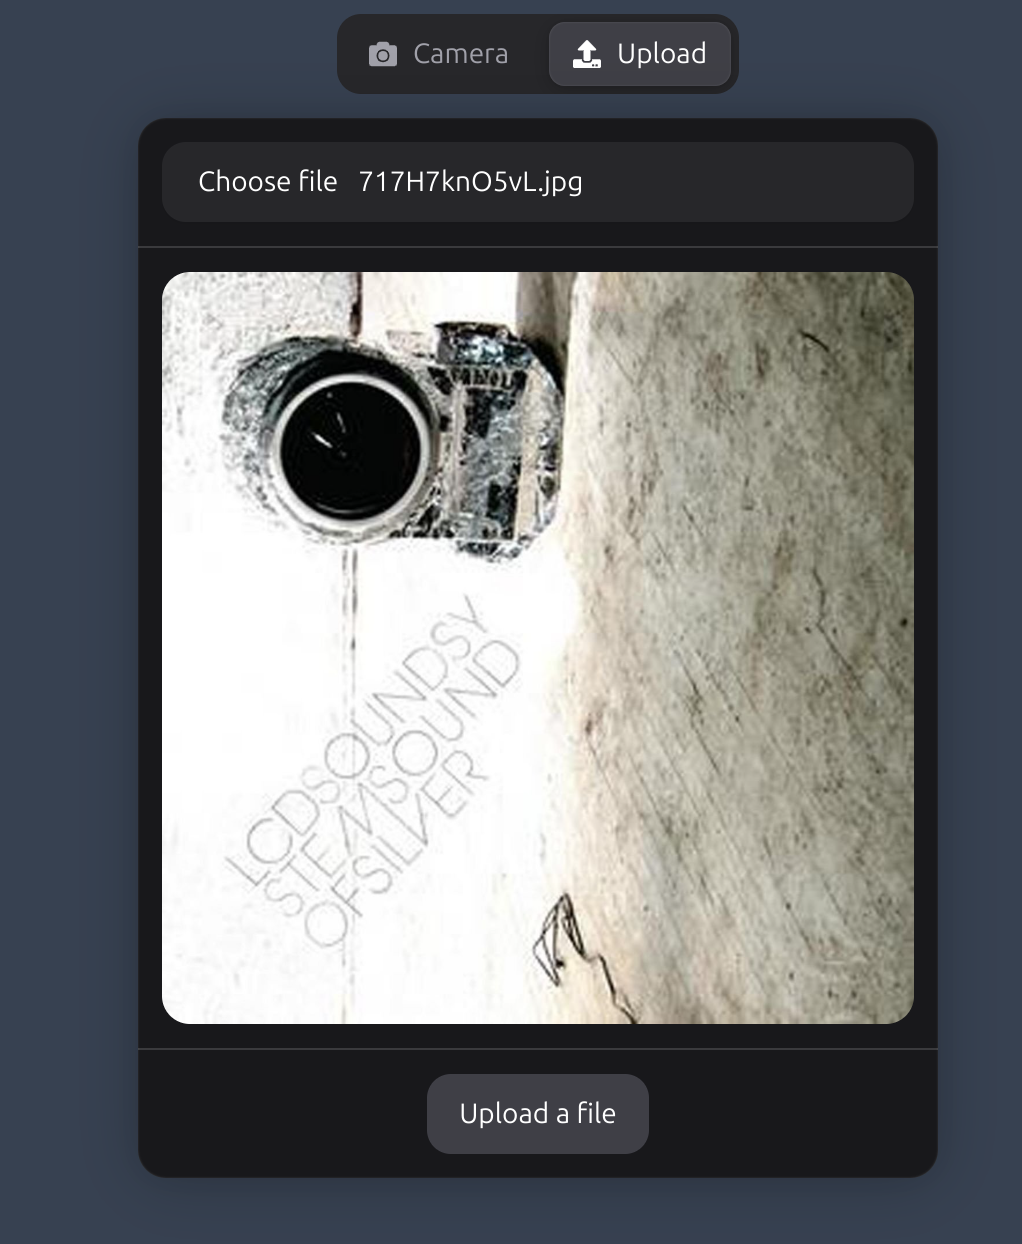
\includegraphics[width=0.4\textwidth]{figures/upload_component.png}
    \caption{The file upload component}
    \label{fig:upload_component}
\end{figure}

\paragraph{Album Collection}
This section remained mainly unchanged from the original design. The user's albums slide across the bottom of the screen, allowing the user to select one by clicking on an album cover. When a user hovers over an album, the sliding is paused, and extra details of that album, such as the title and artist, appear as a tooltip.
A feature added to the original design is the ability to look through the user's collection in a different format, which is also available by clicking the view all button. By pressing this, a modal is opened with all the user's albums in a view reminiscent of flicking through vinyl records in a record store, as seen in Figure~\ref{fig:collection_flick_through}.

\begin{figure} [H]
    \centering
    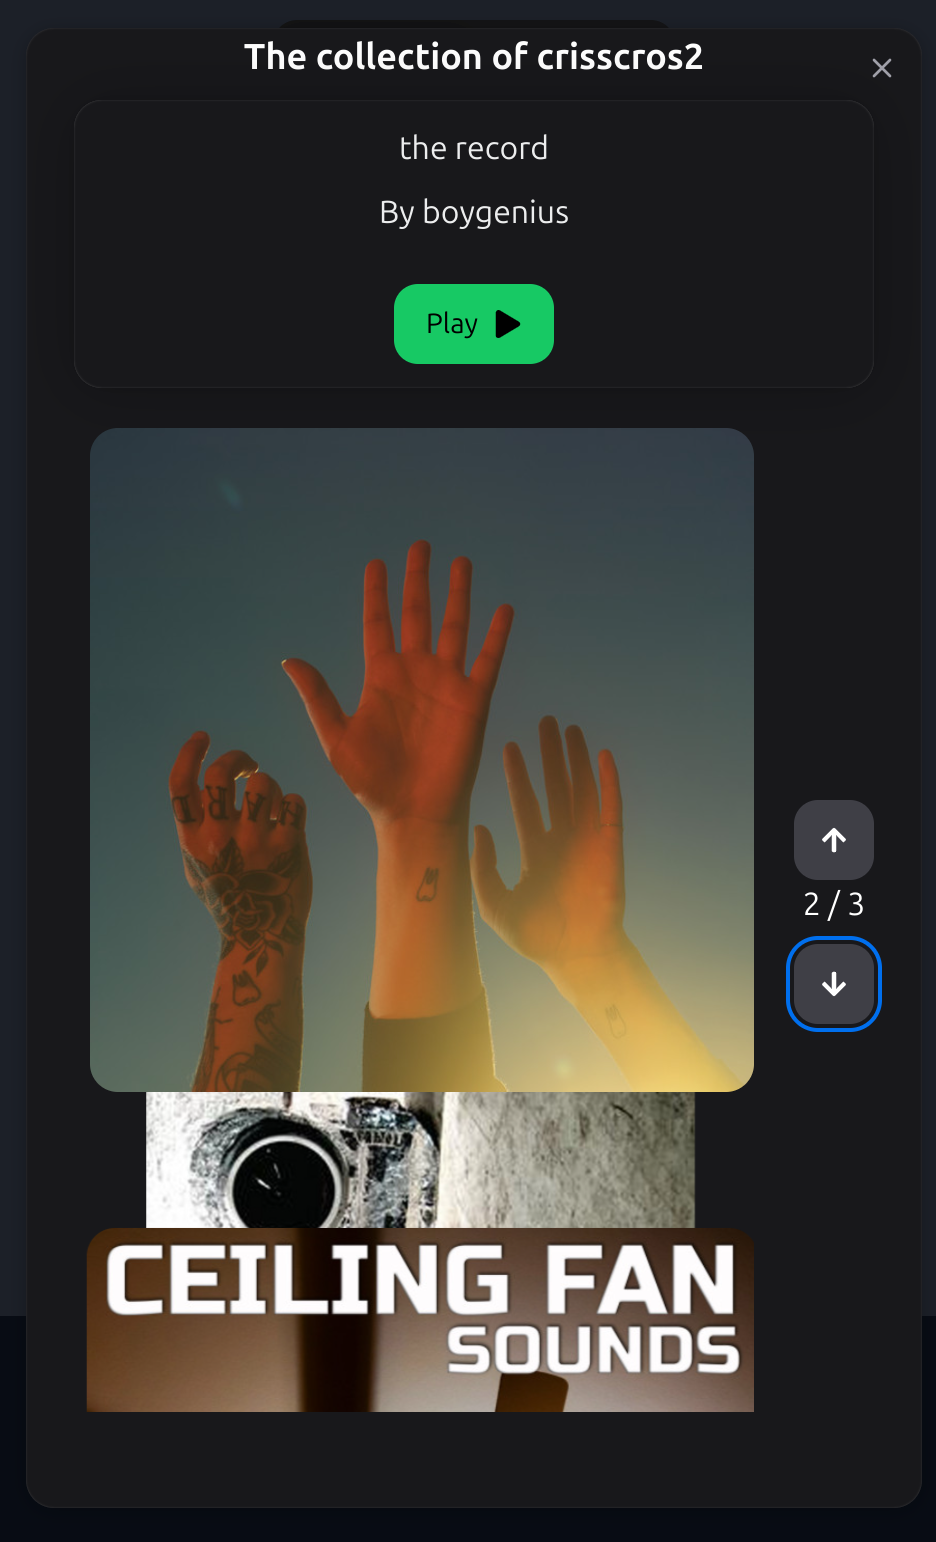
\includegraphics[width=0.3\textwidth]{figures/collection_flick_through.png}
    \caption{The view collection modal}
    \label{fig:collection_flick_through}
\end{figure}

\begin{figure} [H]
    \centering
    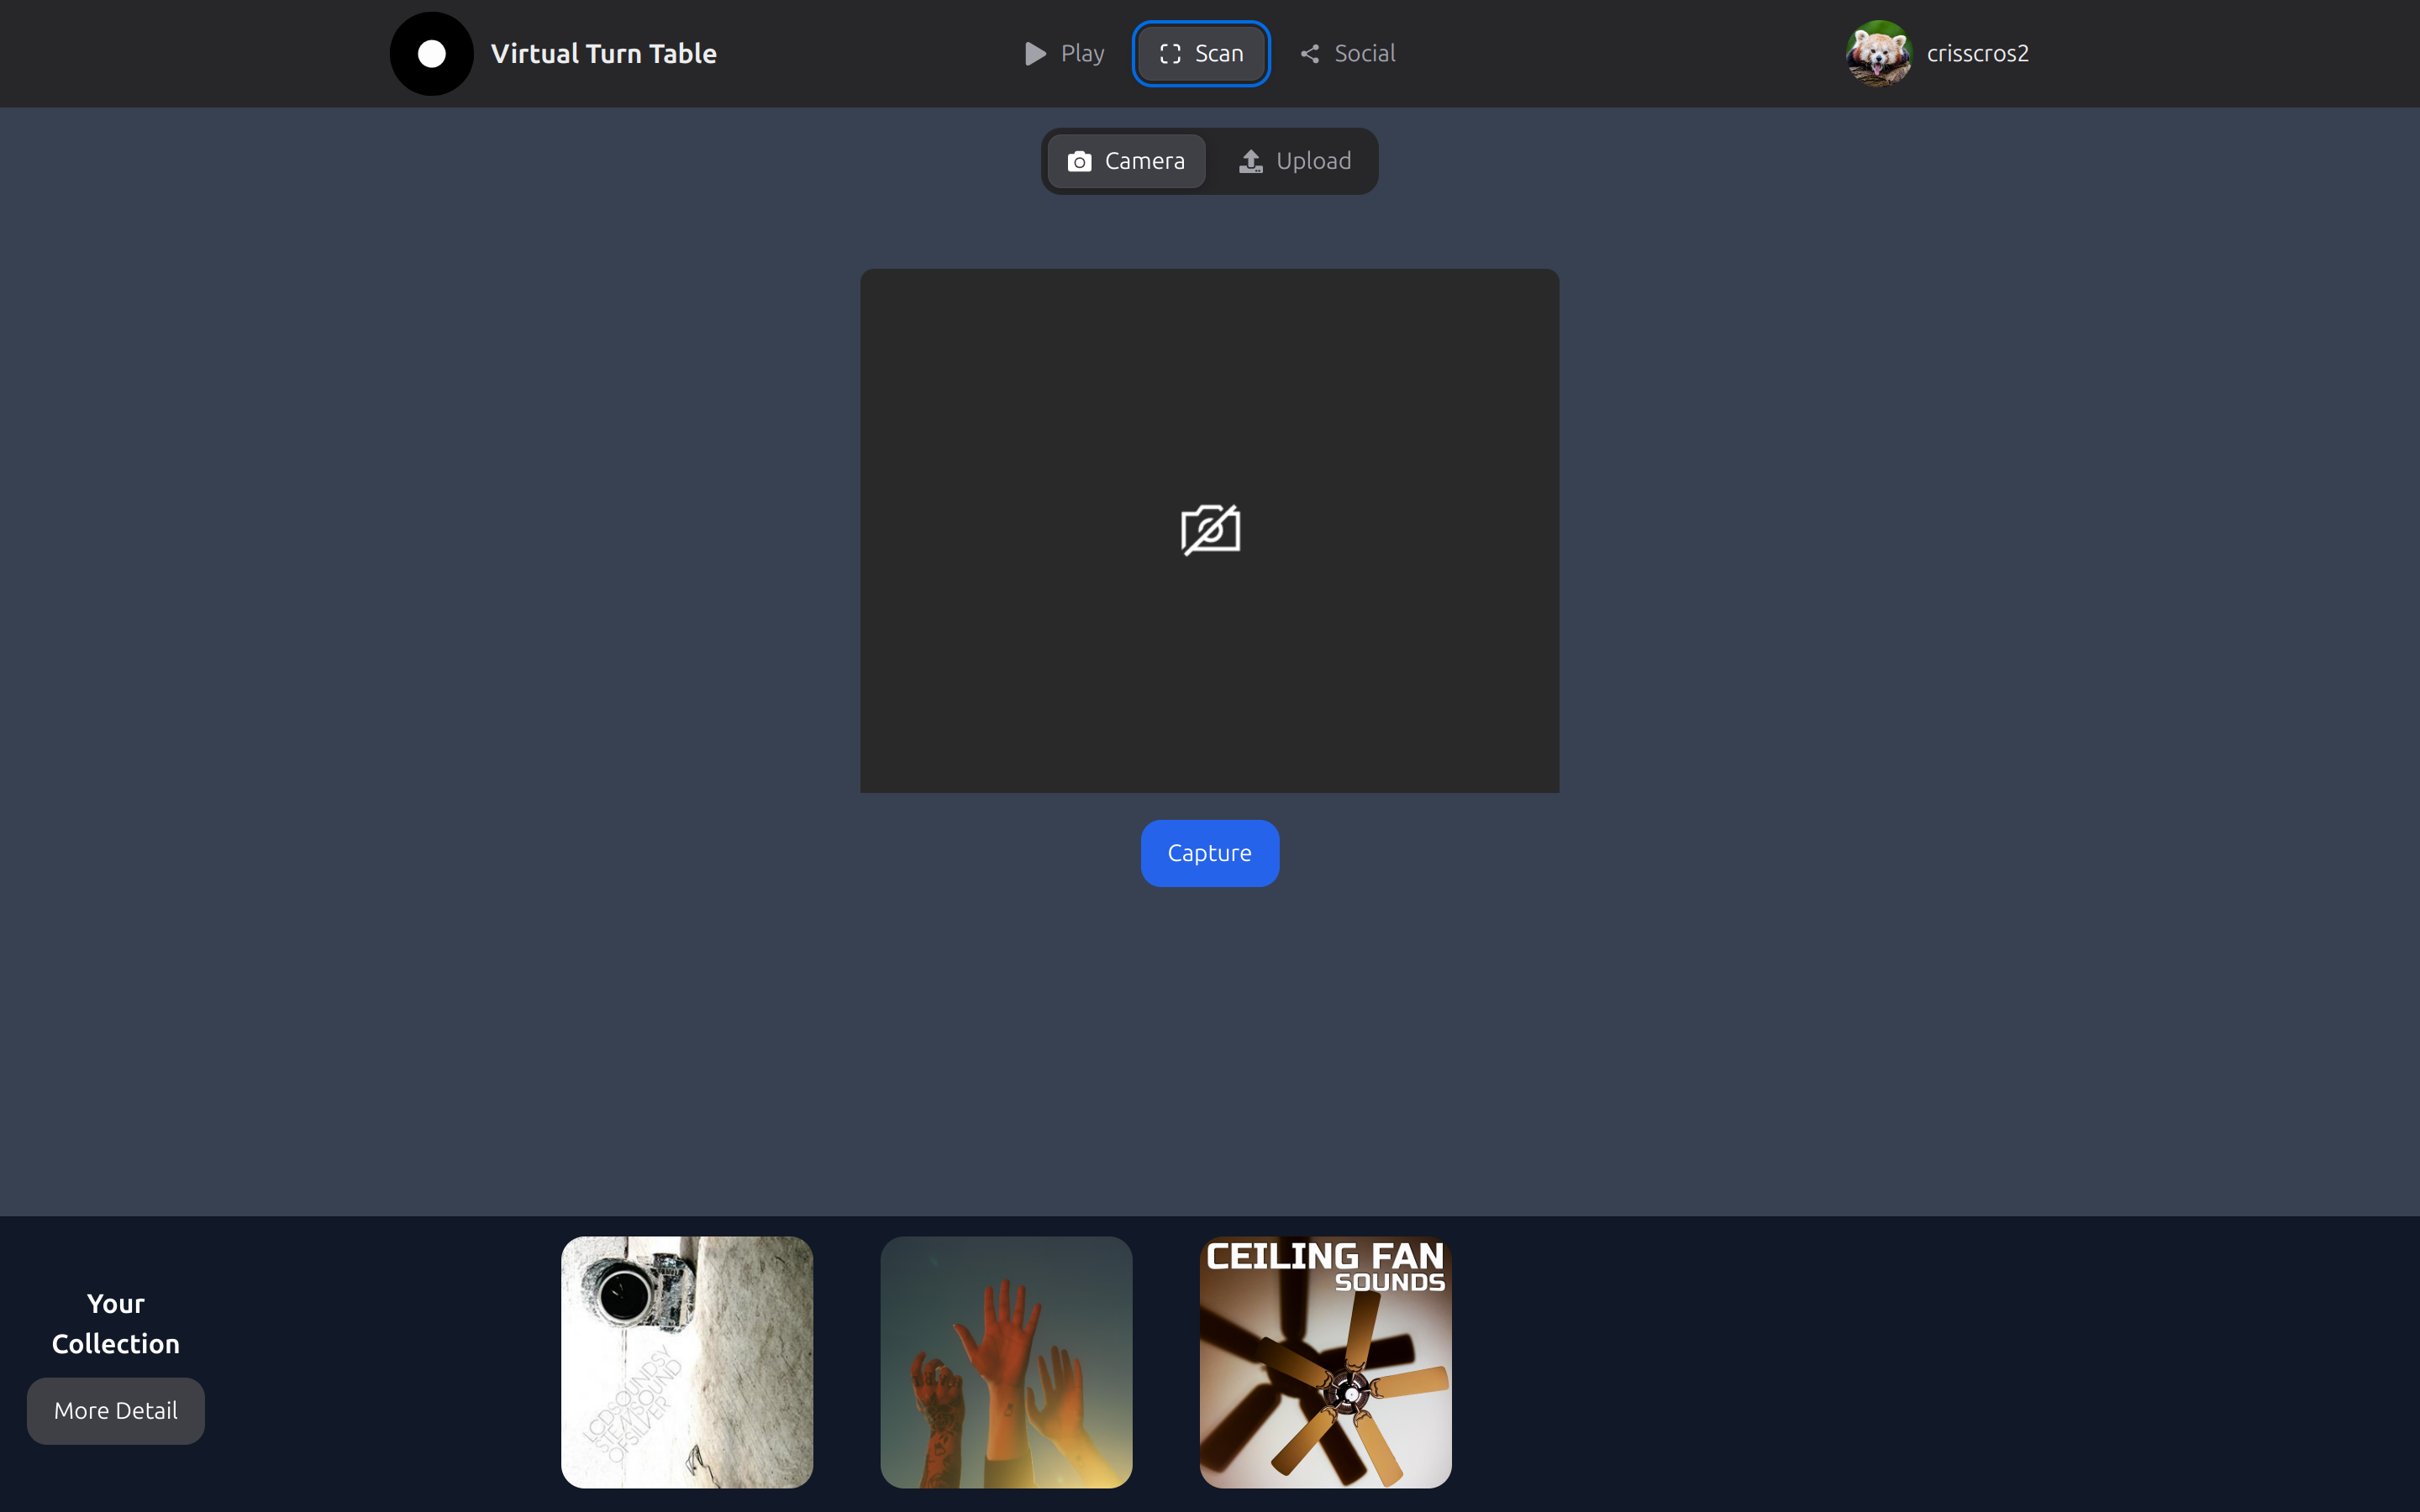
\includegraphics[width=0.8\textwidth]{figures/scan_screen.png}
    \caption{The scan screen of the application with the camera disabled}
    \label{fig:scan_screen}
\end{figure}

\subsubsection{Social Screen}
The social screen had the most significant changes from the original design. Initially, it was implemented as shown in Figure~\ref{fig:social_screen_mockup}, but this layout proved too cluttered, making it challenging to navigate more extensive collections, so a more compact design was needed.

The final design was inspired by the experience of flicking through vinyl records in a record store. Each user's collection is displayed within a grid, where albums pop up and down at random intervals. This approach allows more collections to be visible simultaneously without overwhelming the user.

Additional collections can be loaded incrementally by clicking the 'Load More` button at the bottom of the screen. Users can also explore collections in greater detail by selecting them, which opens the same menu shown in Figure~\ref{fig:collection_flick_through}. The result is that the user is presented with information as it is wanted, a vast improvement over the original design, which filled the screen with too much information for the user to process.

\begin{figure} [H]
    \centering
    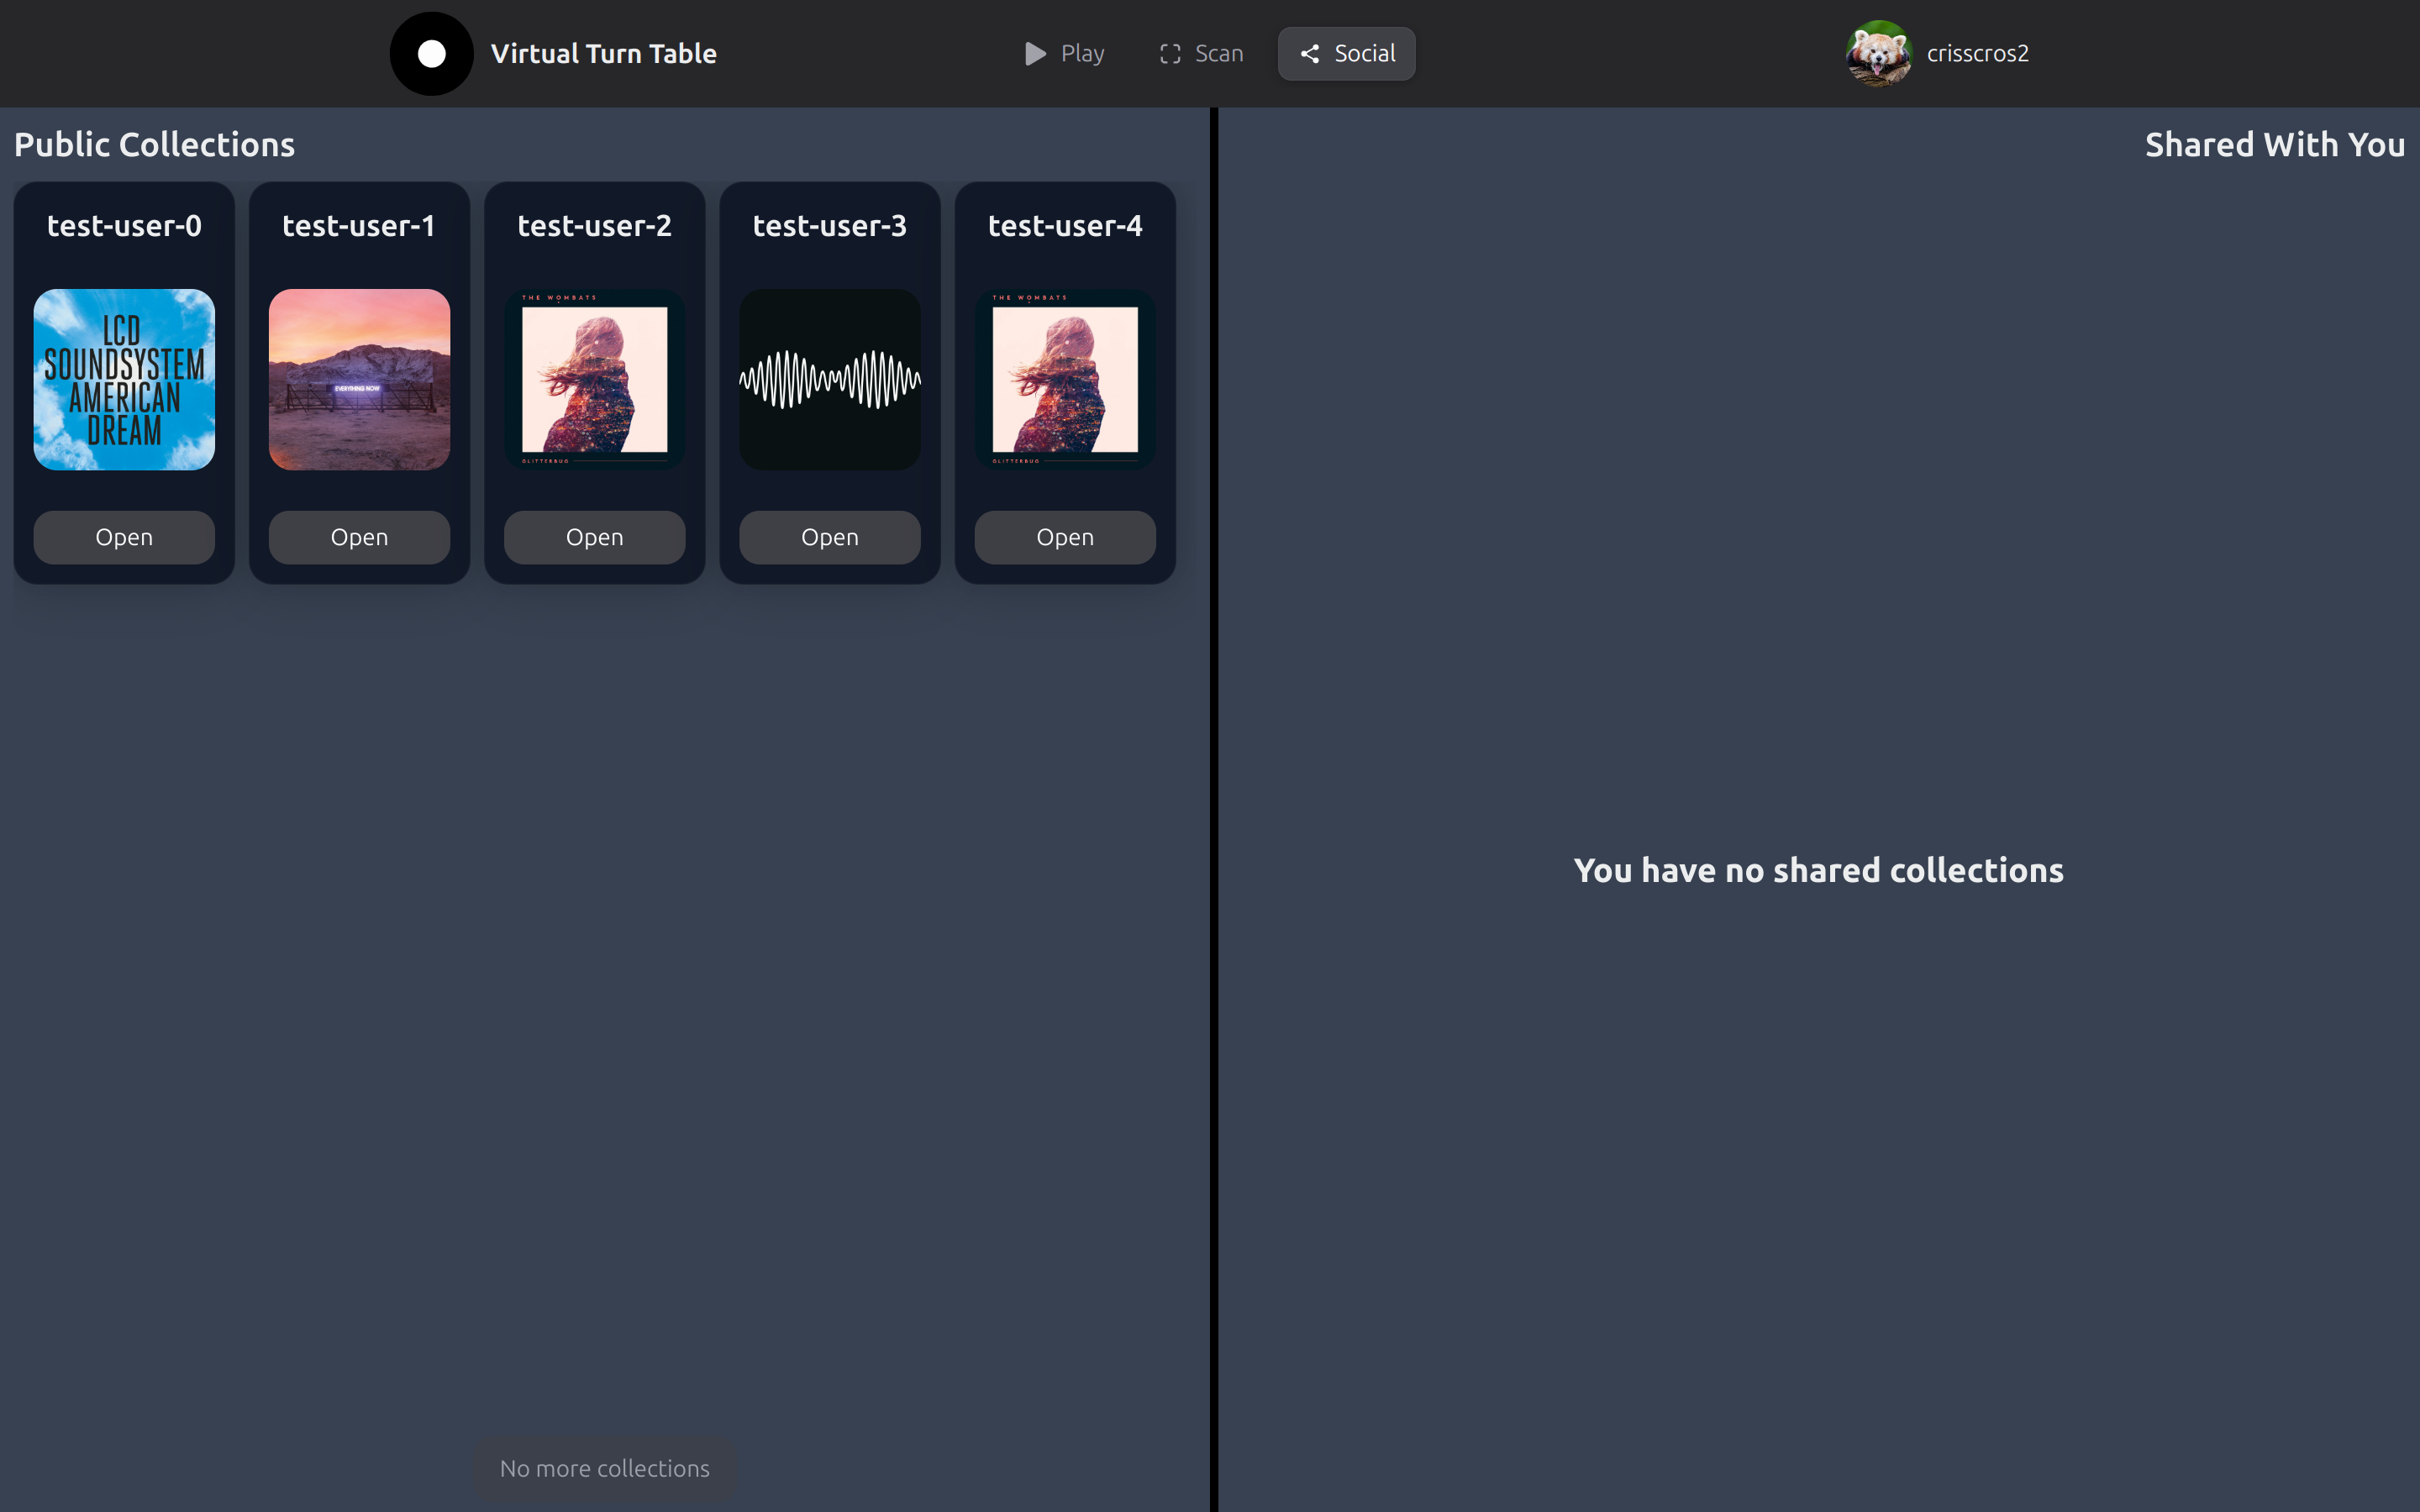
\includegraphics[width=0.8\textwidth]{figures/social_screen.png}
    \caption{The social screen of the application with five public collections}
    \label{fig:social screen}
\end{figure}

\subsection{Automated Testing}
Automated testing of the frontend was carried out using Vitest~\cite{Vitest}, a testing framework designed for projects built with the Vite build system. A test-driven development (TDD) approach was adopted, where test cases were written for each component before the implementation was written. These tests defined the expected component functionality, ensuring that development aligned with predefined functionality. The minimum amount of code is then written to pass these tests, and then further refactoring is made to improve the resulting component. In some cases, test cases themselves required refinement, as unexpected problems necessitated changes in approach for developing specific components. This approach ensured that components did carry out the intended functionality and could be reliably tested in isolation.

The goal for automated testing was to achieve $95\%$ test coverage, ensuring high confidence in the application's functionality. To enforce this, a GitHub Action was configured to run tests on every pull request and push onto the repository's main branch. The build process was set to fail if test coverage dropped below $95\%$ or if any test case failed ensuring these objectives were met.

\subsection{Containerisation}
Containerisation for the frontend involved creating a Docker image that contained a pre-built version of the frontend. Once launched, this would serve the application via an exposed port that users could use to connect.

The application's build itself was straightforward once dependencies were installed. However, these dependencies are not required to be in the Docker image once the build is complete, and since cloud storage has a cost associated with it, the size of the image should be minimised. To achieve this, the following two-stage build process was used:

\begin{description}
    \item[Build Stage] In this stage, a base Node image is used to install all dependencies and then build the application.
    \item[Production Stage] In this stage, the built application is copied from the build stage into a new image. All data not copied from the build stage is left behind, resulting in a much smaller image. This is the image that is then served.
\end{description}

\subsection{Dependency Management}
Frontend dependencies were managed using Node Package Manager (NPM). As new dependencies were installed, a JSON file within the repository was updated to record the package names and their versions. From this file any developer using NPM could install all required dependencies with a single command.

Dependabot, a service provided by GitHub, was integrated into the repository to maintain up-to-date and secure dependencies. Dependabot automatically scanned the dependency file at predefined intervals (e.g., weekly or monthly) and generated pull requests for available updates. This approach ensured that security vulnerabilities were patched and kept all dependencies at their latest versions so the application would not run using deprecated packages. This combined with the automated testing which provided a mechanism to verify whether updated dependencies introduced breaking changes without manual intervention.

\subsection{Challenges}
\paragraph{Environment}
The biggest challenge in frontend development was managing environment variables across different deployment environments. For instance, the BFF URL varied between the development, Docker Compose, and production environments.

This issue was partially solved through dotenv files, which allowed environment variables to be defined in a file and automatically loaded into the application. However, since these files often contained sensitive information, such as API keys, committing to version control was not an option, and so instead, the files had to be managed manually. Despite this limitation, once the dotenv files were properly set up, the approach functioned reliably across deployments.

\paragraph{Spotify API Changes}
Midway through development, Spotify updated their authentication flow to require HTTPS for redirect URLs, disabling non-HTTPS redirects~\cite{spotifyredirects}. The cloud deployment was unaffected, as it already used HTTPS. However, the development environment did not, which broke the authentication flow when running locally. Fortunately, there was an easy fix: the services were just launched using self-signed SSL certificates. Though the impact on the project was small, this change highlights the risks of relying on external services and the potential for breaking changes.

\paragraph{Maintaining State Between Refreshes}
The local state of the frontend is managed through variables that are reset upon page refreshes. As a result, if a user refreshes the page or closes the browser and reopens it, the session is lost, requiring them to repeat logging in and selecting or scanning an album. This issue was solved by storing state data in the browser's local storage. When the application initialises, it attempts to retrieve stored session data. The session is restored if valid data is found, allowing the user to continue from where they left off or reset to the landing page if none is found. The result is if users refresh the page while listening to an album, they are returned to the play screen with the same album and song still playing.

\section{Backend}~\label{sec:backend-development}
\subsection{Implementation}
Each backend service followed a similar implementation structure, consisting of a FastAPI application responsible for serving API endpoints. Depending on its functionality, each service could also establish WebSocket connections or interact with a database.

All three services included two basic endpoints:
\begin{description}
    \item[Health Check:] A health check endpoint to monitor service availability, useful for checking if a service started correctly.
    \item[Docs Redirect:] A redirection endpoint leading to the automatically generated API documentation (removed in the deployed version).
\end{description}

To better organise the API, each service was structured using routers to categorise endpoints into logical sections, such as authentication or user data retrieval. This modular approach improved API organisation, making it easier to understand and use.

\subsubsection{BFF}
The Backend for Frontend (BFF) service was structured into five distinct routers, each responsible for a specific aspect of the application:

\begin{description}
    \item[Music Router:] Handles all endpoints related to music playback and retrieving album or song data.
    \item[User Router:] Manages user-related endpoints, including user data retrieval and updates.
    \item[Image Search Router:] Facilitates communication with the image-to-album service, handling album identification from uploaded images.
    \item[Authentication Router:] Manages user authentication, including login and token validation.
    \item[Social Router:] Handles endpoints related to social functionality, such as collection sharing and retrieving shared collections.
\end{description}

Additionally, the BFF manages the WebSocket functionality for the notification system. A WebSocket connection is established between the frontend and the BFF when a user logs in. If a collection is shared with the user, the BFF asynchronously sends a notification via the WebSocket connection, prompting the frontend to display the new notification to the user.

\subsubsection{User Data Service}
The User Data Service was the most complex of the three backend services, requiring direct interaction with a database. SQLAlchemy was used as an Object Relational Mapping (ORM) tool to manage database interactions, with each database table defined as a class in the code. The result of this is that items in the database are treated as objects in the code making manipulation of the data easier and less error-prone than using raw SQL queries.

The service was structured into two primary routers:

\begin{description}
    \item[User Router:] Handles all endpoints related to individual users.
    \item[Social Router:] Manages endpoints related to social functionality, including collection sharing and retrieval.
\end{description}

Alembic, a database migration tool, ensured data was not lost during database schema changes. Once a change is made to the schema Alembic automatically generates migration files that could be executed to update the database schema while preserving existing data. Although this was not a critical concern during development since no real user data was stored, such a system would be important in a production environment, where data persistence must be maintained across schema updates.

\subsubsection{Image To Album Service}
The Image-to-Album Service was the simplest of the three backend services, consisting of only two routers, each containing a single endpoint:

\begin{description}
    \item[Image Processing Router:] Handles the conversion of an uploaded image into a predicted album match.
    \item[Album Retrieval Router:] Retrieves the corresponding Spotify album ID based on the predicted album match.
\end{description}

This service was stateless, so it did not require persistent data storage between requests.

The first guess was implemented using the best guess functionality of the Google Reverse Image Search API. This would then be run through the Spotify search API, which would return an album that would be displayed to the user.

The scattershot approach used separate data from the best guess reverse image search. Instead, it would look at the websites that matched the image and then use the page's title as a search term. The hope was that this would prove effective because music albums are often the subject of reviews and sales pages containing the album title.

Any other techniques for identification of albums could be implemented as different endpoints in these two routers, allowing for easy expansion of the service's functionality. For example, a barcode scanner could be implemented as a separate endpoint in the Image Processing Router, which would return some data that could then be run through the Album Retrieval Router to get the Spotify album ID.

\subsubsection{Security}~\label{sec:backend-security}
Security measures were implemented differently across the three backend services to ensure proper control over data access.

For the User Data Service and Image-to-Album Service, middleware enforced security by rejecting all requests not originating from the BFF service, ensuring only authentic and validated requests from the BFF could interact with these services.

The BFF required a more complex security approach, as it had to handle requests from external users. To perform authentication, JSON Web Tokens (JWTs) were used, which are common in web applications~\cite{9320801}. When a user logs in via Spotify, the frontend sends that token to the backend. If the token is valid, the backend issues a JWT formed from the given token and the user's username; this is then included in the headers of subsequent requests to the BFF.

This token-based authentication ensures that users can only access their own data and that requests without a valid JWT are rejected, preventing unauthorised access.

\subsection{Automated Testing}
Automated testing for the backend was carried out using the Pytest library~\cite{PyTest}, which allows for creating custom test fixtures to set up and tear down the environment for each test, including managing the database state. FastAPI provides a test client that was utilised to simulate calls to endpoints to be tested as if an actual client was calling the endpoints.

Extensive use of mocking was necessary for simulating external API calls. Mocking was especially important in the BFF service, which made numerous calls to the other two backend services. It ensured that each service could be tested in isolation without requiring live responses from the other services and external APIs, making the testing process more reliable and efficient.

\subsection{Containerisation}
The three backend services were containerised using an Alpine Linux image with Python pre-installed. Alpine Linux was chosen as it is one of the smallest available Linux distributions, reducing the cost of storing the image in a cloud artifactory, along with a focus on security, so vulnerabilities in the base image itself were far less likely.

Unlike the frontend, where dependencies are only needed during the build process, the backend dependencies must be present at runtime for the services to function correctly. As a result, a multi-stage build was not used. Instead, dependencies were installed in the same stage as the application files were copied into the container image, ensuring all required packages were available when the service was deployed. This approach's disadvantage is that the image size is larger, but this is unavoidable due to the nature of the backend services.

\subsection{Dependency Management}
Unlike Node applications, Python does not have a standardised dependency management system. Multiple tools, such as Pipenv and Poetry, can be used. For simplicity, the solution chosen for this project was a requirements.txt file, which lists all dependencies using semantic versioning. This approach allows dependencies to be installed using pip, the most widely used Python package manager, with a single command.

Dependency updates were managed similarly to the frontend. Dependabot was configured to scan the requirements.txt file regularly, generating pull requests for available updates. These updates followed the same schedule as frontend dependencies, ensuring that the dependencies were kept up to date and security vulnerabilities were patched as soon as possible.

\section{Code Quality}~\label{sec:code-quality}
Code quality standards were maintained during development through pre-commit hooks and GitHub Actions. Pre-commit hooks were configured to run linters and formatters before code was committed to the repository. This ensured potential issues were identified early, preventing poor-quality code from getting pushed into the repository. This approach was particularly valuable since a single developer developed the project, so there was no code review process to catch mistakes.

In addition to the pre-commit hooks, automated tests and security scans were executed every time a pull request was created or a commit was pushed to the repository's main branch. While these checks could have been integrated into the pre-commit hooks, this was avoided due to the tests' execution time, which would have led to a tedious development process. Instead, the tests were run on GitHub servers, leveraging parallel execution to reduce the overall testing time.

\section{Challenges}
\subsection{Database Testing}
Testing the user data service required running functions that directly interacted with a database. The challenge here is mocking the database would be difficult and a bad representation of the actual database. So a test database setup had to be used and its state had to be managed while the tests were running. Each test had to run in a state that was completely independent of others else the tests might exhibit flaky behaviour. The only way to get around this would be to provide a connection to each test that would appear to be a clean database and once the test was complete roll back any changes made to the database.
